%
%   Data Clarification
%       - Plots...
%   
\clearpage
\section{Data clarification}
\label{section:data_clarify}








\subsection{Overview of attributes}

In this section, we provide a big picture of the our data via visualizations.

\subsubsection{Categorical attributes}

\begin{figure}[H]
    \centering
    \begin{subfigure}[b]{0.49\textwidth}
        \centering
        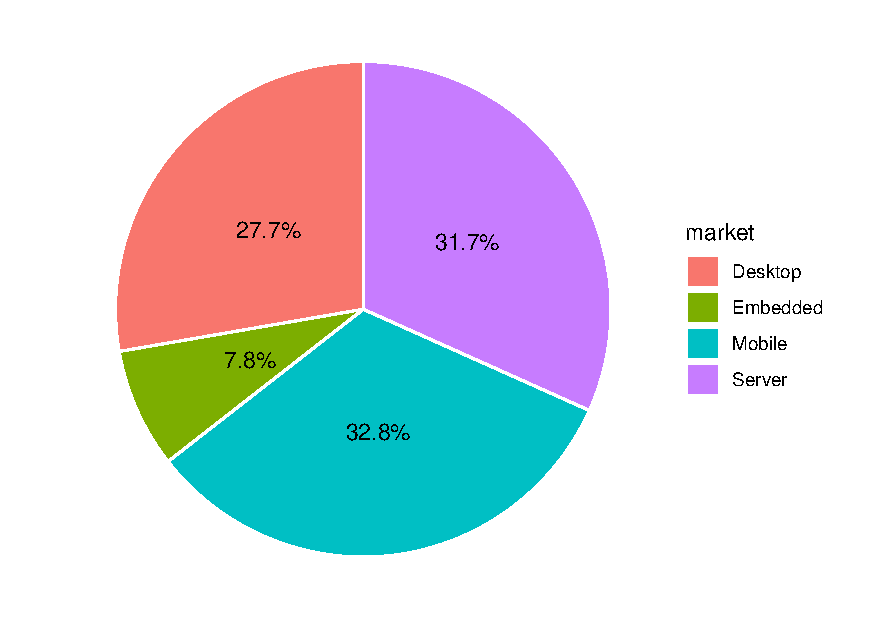
\includegraphics[width=\textwidth]{./graphics/pie_market.pdf}
        \caption{Pie of market share}
    \end{subfigure}
    \hfill
    \begin{subfigure}[b]{0.49\textwidth}
        \centering
        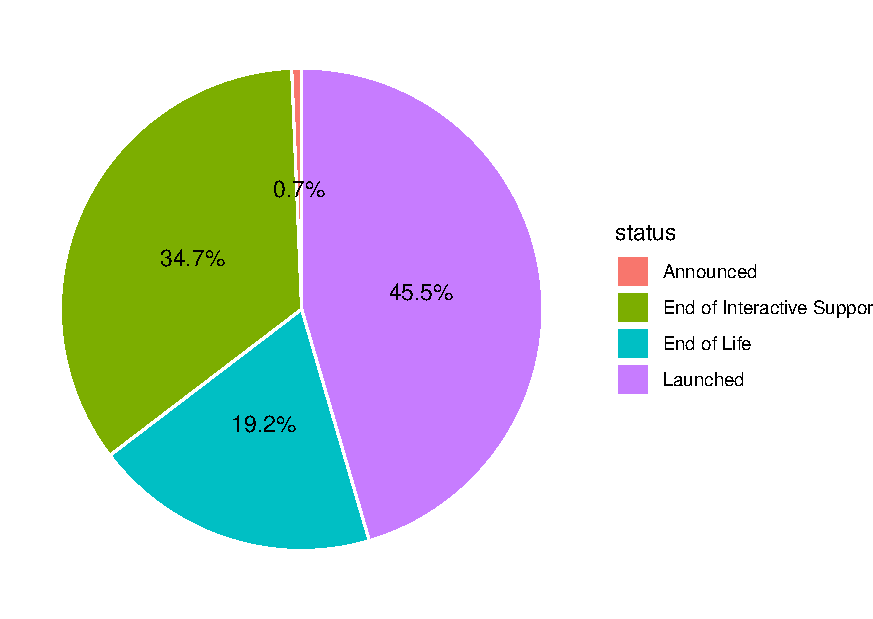
\includegraphics[width=\textwidth]{./graphics/pie_status.pdf}
        \caption{Pie of status}
    \end{subfigure}
    \caption{Pies of categorical attributes}
    \label{fig:pie_category}
\end{figure}

\inputcode[firstline=59,lastline=73]{R}{rcode/clarification.rmd}

\textbf{[Figure \ref{fig:pie_category}]} Two obvious categorical attributes of our data are \textit{Market} and \textit{Status}.
\begin{itemize}
    \item In \textit{Market} attribute, three primary shares of market are Desktop, Server and Mobile. Embedded constitues a very small
    proportion.
    \item In \textit{Status} attribute, most of them are Launched, End of Life or End of interactive support. A tiny amount of Announce
    contributes modestly to total amount of CPU's model by provider Intel.
\end{itemize}

In terms of the code we used to plot two above pies. Each line is self-explanatory. Since two pies have different configurations, and would be
verbose to explain everything here, we leave the detailed implementation in \verb|rcode/clarification.rmd|. A few things to note are:
\begin{itemize}
    \item \verb|data_percentages| is a data-frame containing three properties: \verb|market|, \verb|value| and \verb|percent|.
    Note that, we use variable \verb|market| two times: one for plotting market-pie and one for plotting status-pie. This is just for ease
    of use and avoid repeating the code. It should not be taken seriously (the same name for two different things could be confusing).
    \item \verb|market| are the levels of \verb|market|-attribute (or \verb|status|-attribute)
    \item \verb|value| is the vector of frequencies of each \verb|market| (or \verb|status|)
    \item \verb|percent| is the vector percentages (computed by dividing the frequency by total and multiply by $100$)
\end{itemize}





\subsubsection{Continuous attributes}

\begin{figure}[H]
    \centering
    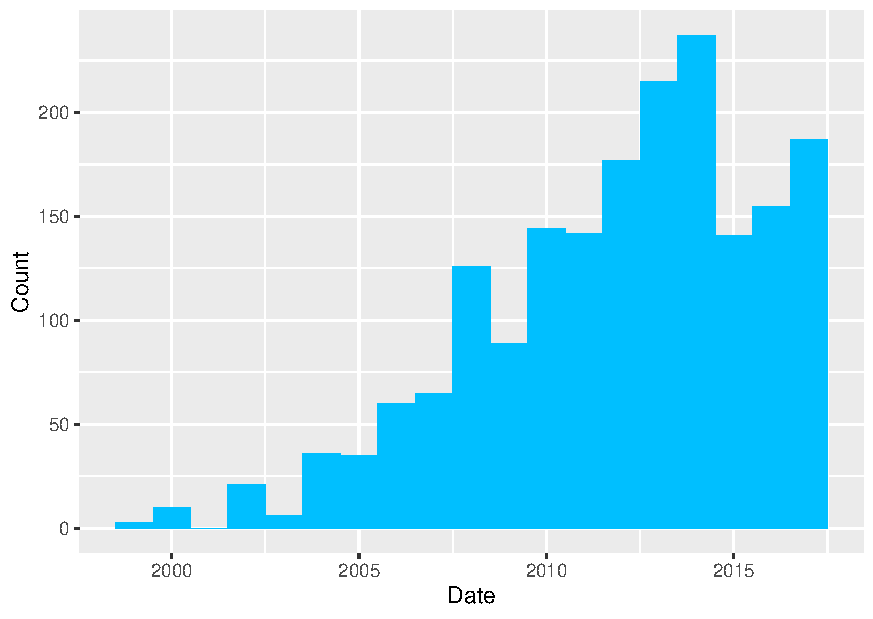
\includegraphics[width=0.5\textwidth]{./graphics/hist_ldate.pdf}
    \caption{Histogram of launch date}
    \label{fig:hist_ldate}
\end{figure}

\inputcode[firstline=78,lastline=80]{R}{rcode/clarification.rmd}

\textbf{[Figure \ref{fig:hist_ldate}]} The \textit{Launch date} histogram shown that most of Intel's CPUs are launched recently, with two notable peaks at 2014 and 2017. The legacy
CPUs (before 2005) are only minor and can be treated as outliners if it is used in further analysis.






\begin{figure}[H]
    \centering
    \begin{subfigure}[b]{0.49\textwidth}
        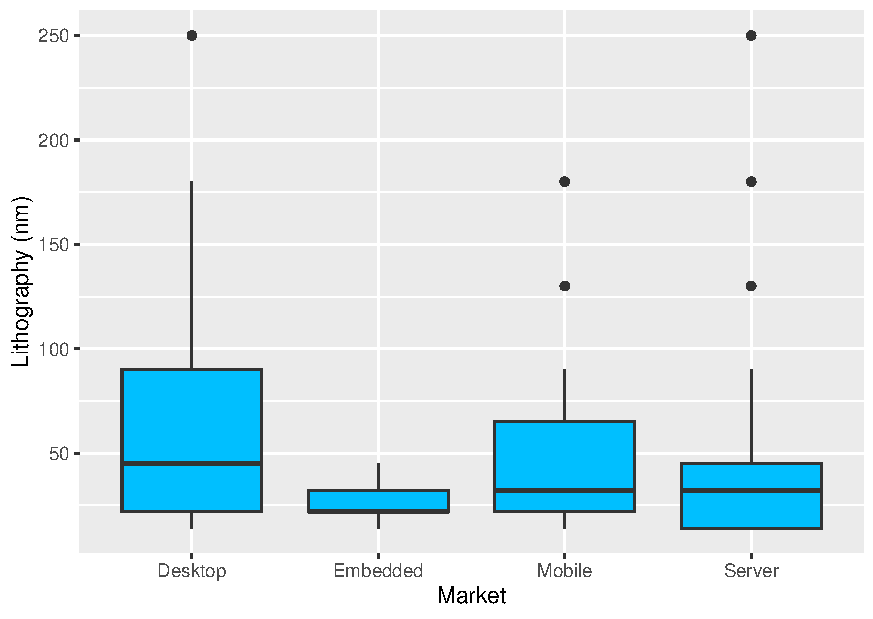
\includegraphics[width=\textwidth]{./graphics/box_litho.pdf}
        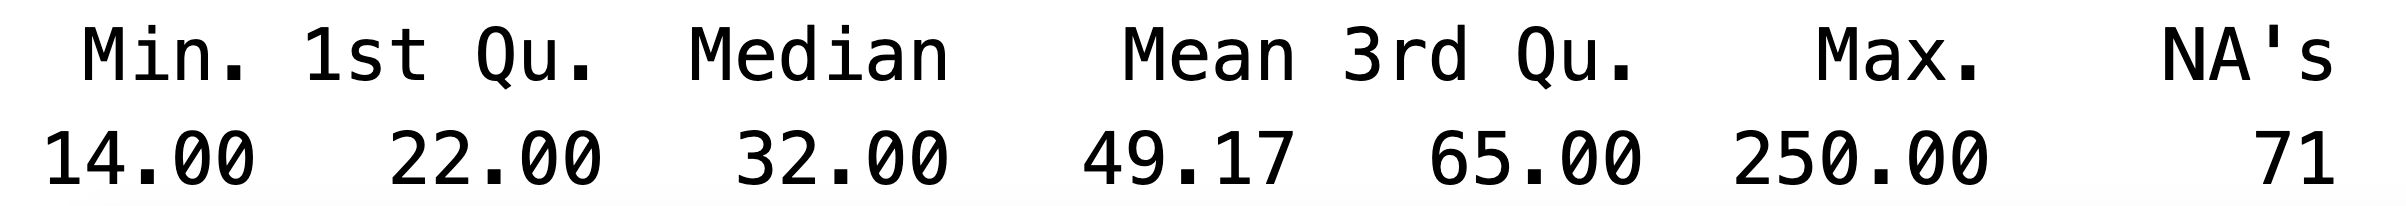
\includegraphics[width=\textwidth]{./graphics/sum_litho.png}
        \caption{Box plots and Summary of Lithography}
        \label{fig:box_litho}
    \end{subfigure}
    \hfill
    \begin{subfigure}[b]{0.49\textwidth}
        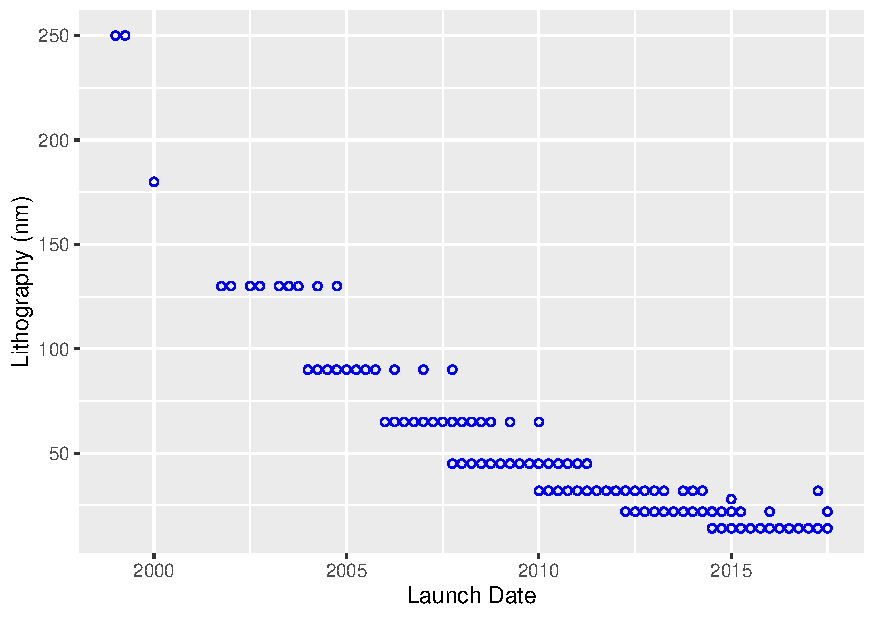
\includegraphics[width=\textwidth]{./graphics/scatter_litho.pdf}
        \caption{Plot of lithography over time.}
        \label{fig:scatter_litho}
    \end{subfigure}
    \caption{Lithography plots}
\end{figure}

\inputcode[firstline=85,lastline=89]{R}{rcode/clarification.rmd}

\inputcode[firstline=94,lastline=96]{R}{rcode/clarification.rmd}

\textbf{[Figure \ref{fig:box_litho}]} The box plot of \textit{Lithography} (chip printing technique) demonstrates interesting characteristics:
\begin{itemize}
    \item There was a large variance in the types of Lithography designed in Intel's Desktop processors, a smaller, but significant variance of 
    Mobile and Server are also observed. Embedded is less diverse, however, and also concentrates mostly on small \textit{Lithography} printings.

    \item The mean of \textit{Lithography}, in whatever market, is also approximately the same. That number might represents the most suitable 
    printing technique that is widely used among Intel's CPUs.
\end{itemize}

Overall, the most common \textit{Lithography} is $32 nm$. The best printing technique possible was $14 nm$ and the worst was $250 nm$. That large
number might come from old, legacy processors which were not designed with recent innovations in the Chip industry.

\textbf{[Figure \ref{fig:scatter_litho}]} The scatter plot of \textit{Lithography} with respect to \textit{Launch date} shown that the lithography
is getting smaller over time, and they are categorized into specific groups. So \textit{Lithography} can be treated as a Categorical attribute as well
as Continuous attribute.







\begin{figure}[H]
    \centering
    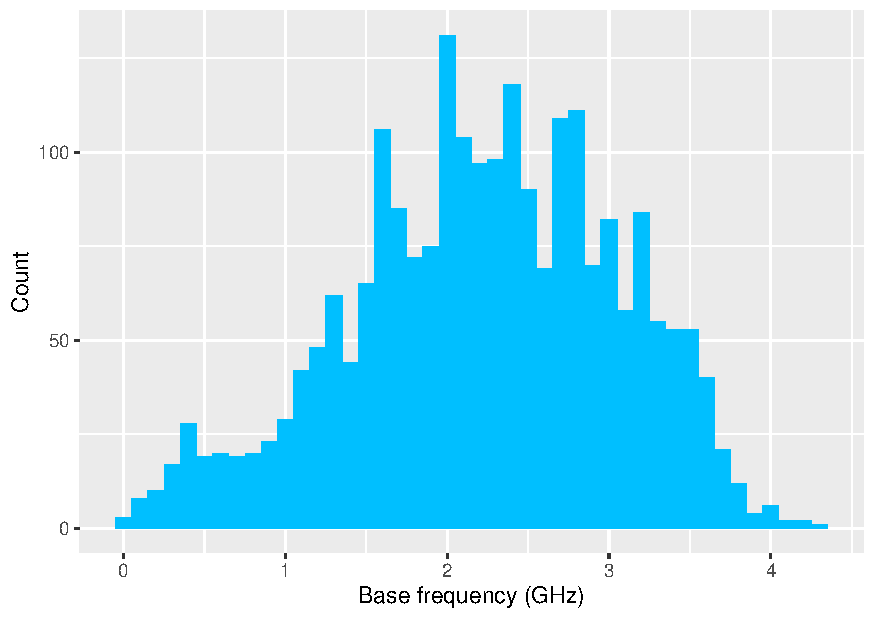
\includegraphics[width=0.5\textwidth]{./graphics/hist_bfreq.pdf}
    \caption{Histogram of Base Frequency}
    \label{fig:hist_bfreq}
\end{figure}

\inputcode[firstline=108,lastline=110]{R}{rcode/clarification.rmd}

\textbf{[Figure \ref{fig:hist_bfreq}]} The most significant trend that could be observed in the \textit{Base frequency} histogram is its "normality".
In fact, this is expected because though higher frequency results in better performance, it has power and heat trade-offs. Thus, we see most choices of
frequencies concentrate around the mean of the distribution, which look pretty much like a bell-shape. We will discuss this property again in the Regression
section.






\begin{figure}[H]
    \centering
    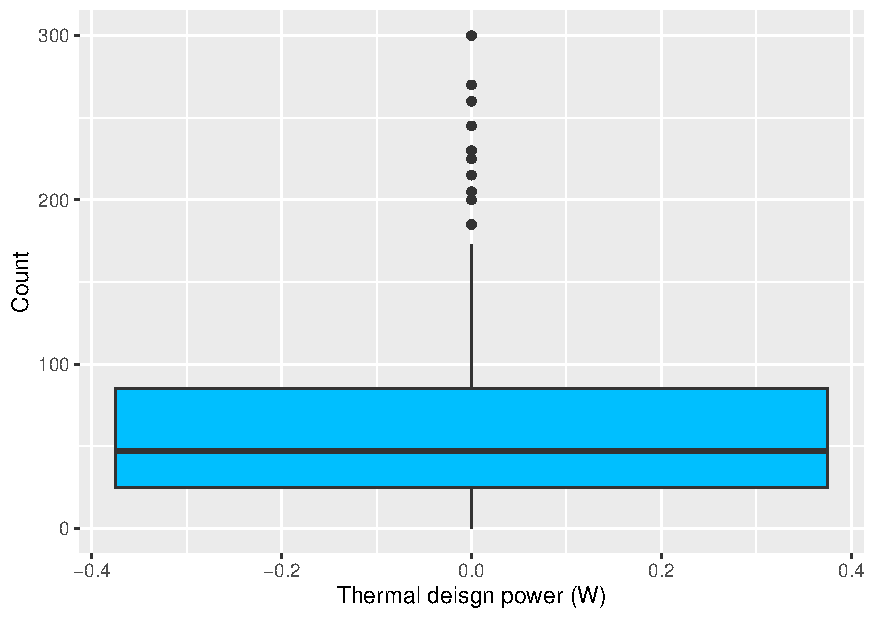
\includegraphics[width=0.5\textwidth]{./graphics/box_tdp.pdf}
    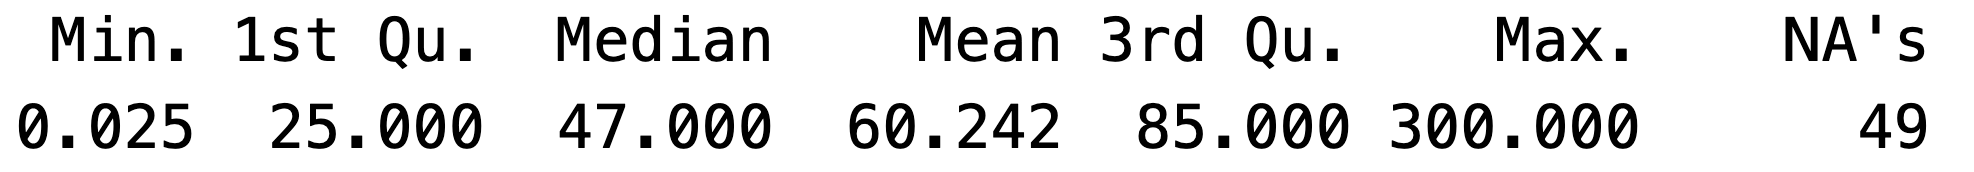
\includegraphics[width=0.5\textwidth]{./graphics/sum_tdp.png}
    \caption{Box plots and Summary of Thermal Design Power}
    \label{fig:box_tdp}
\end{figure}

\inputcode[firstline=115,lastline=119]{R}{rcode/clarification.rmd}

\textbf{[Figure \ref{fig:box_tdp}]} The box plot of \textit{Thermal design power} is very market-dependent. While Embedded needed a very decent amount of
energy to release the heat, Server needed a lot, which is demonstrated by a much higher median. Server TDP's variance is also large, indicating
that there are many choices within this market. However, even so, its first quantile is still larger than most of the CPUs used in other markets.





% Should we plot memory bandwidth?
% \begin{figure}[H]
    %\centering
    %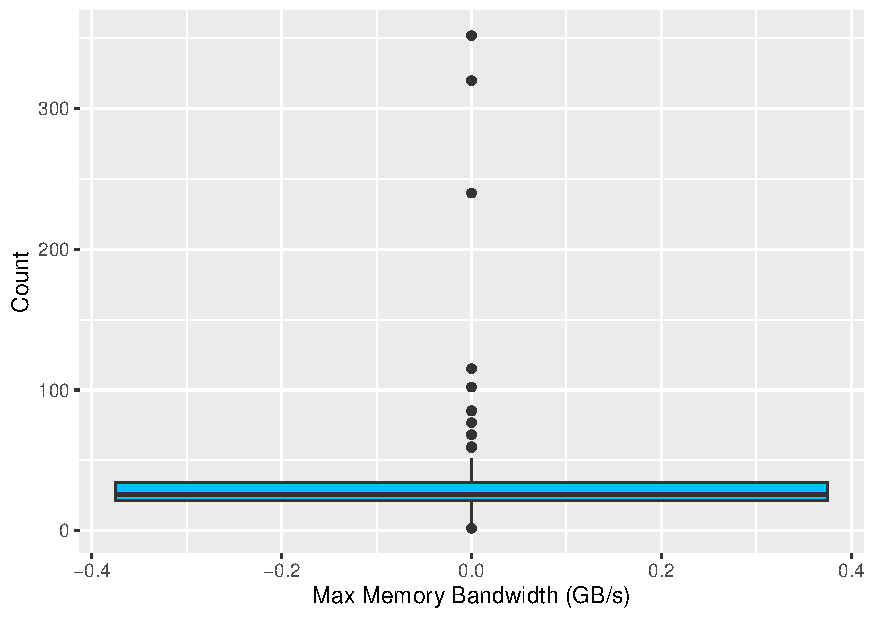
\includegraphics[width=0.5\textwidth]{./graphics/box_memband.pdf}
    %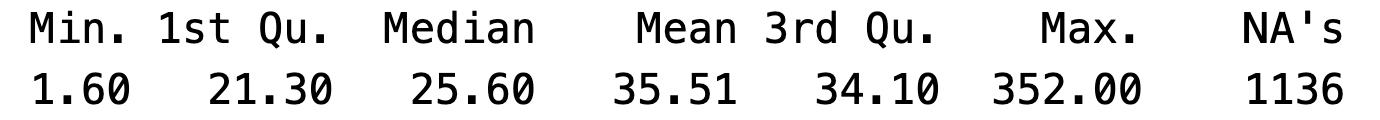
\includegraphics[width=0.5\textwidth]{./graphics/sum_memband.png}
    %\caption{Histogram of Maximum Memory Bandwidth}
%\end{figure}





% Should we plot Temperature? 
%\begin{figure}[H]
    %\centering
    %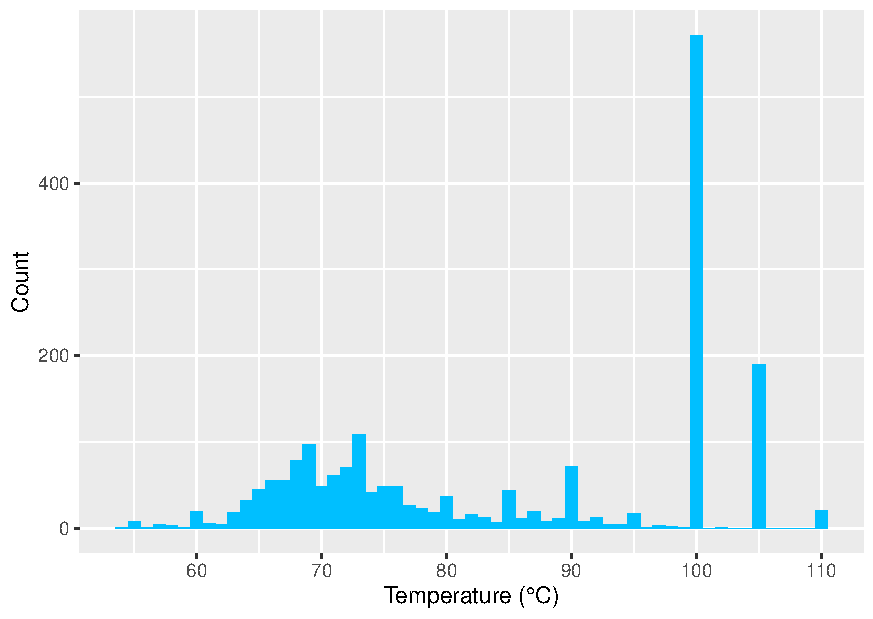
\includegraphics[width=0.5\textwidth]{./graphics/hist_temp.pdf}
    %\caption{Histogram of Temperature}
    %\label{fig:hist_temp}
%\end{figure}









\subsection{Analysis of attributes}

In this section, we emphasize key relationships of our interest. The following plots will be reused in later parts of our report. The reasons why we paid our
attention on these attributes will be discussed in \textbf{Section \ref{section:data_analysis}}.



\subsubsection{Base frequency with respect to Lithography and Number of Cores}

Firstly, focusing on the previous Lithography plot \textbf{[Figure \ref{fig:scatter_litho}]}, we can see that they are well categorized into particular groups.
That speaks well for the reality, since there were not so much CPU printing techniques on the market.
Thus, we can choose the represent this attribute as a categorical variable.

We plot the distribution of \textit{base frequency} for each category of \textit{Lithography} as follows:

\begin{figure}[H]
    \centering
    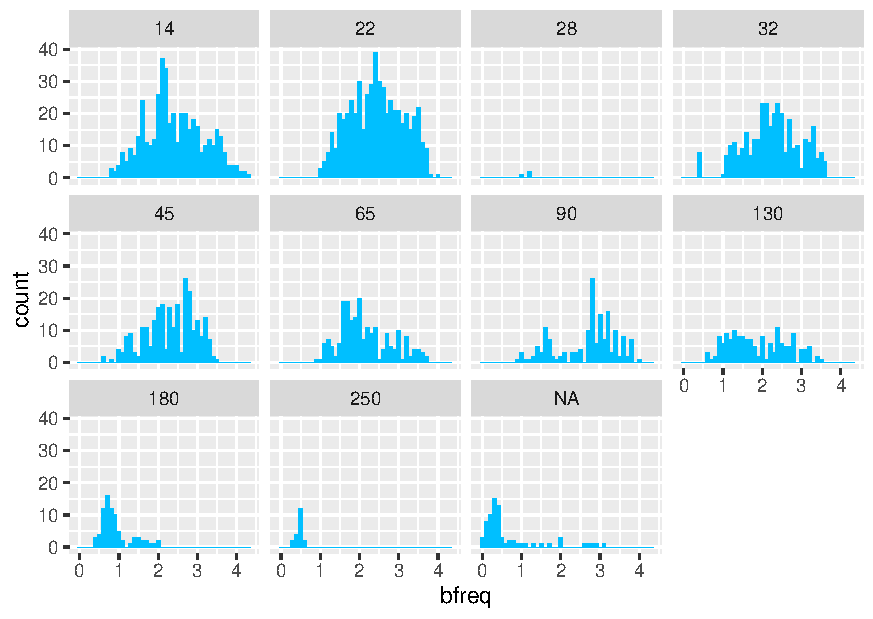
\includegraphics[width=0.5\textwidth]{./graphics/hist_bfreq_wrt_litho.pdf}
    \caption{Base frequency distribution of each Lithography}
    \label{fig:hist_bfreq_wrt_litho}
\end{figure}

%\inputcode[firstline=115,lastline=119]{R}{rcode/clarification.rmd}
\textbf{NOTE: THERE IS A CODE REFERENCE HERE}

We observed that some categories are not significant in terms of quantity, and large lithography ($> 45$) might come from old, obsolete CPUs. We choose
only \verb|14, 22, 32, 45| and ignore the rest.

\textbf{NOTE: THERE IS A CODE REFERENCE HERE}

Secondly, we would like to see the relationship between \textit{Number of cores} and \textit{Base frequency}.

\begin{figure}[H]
    \centering
    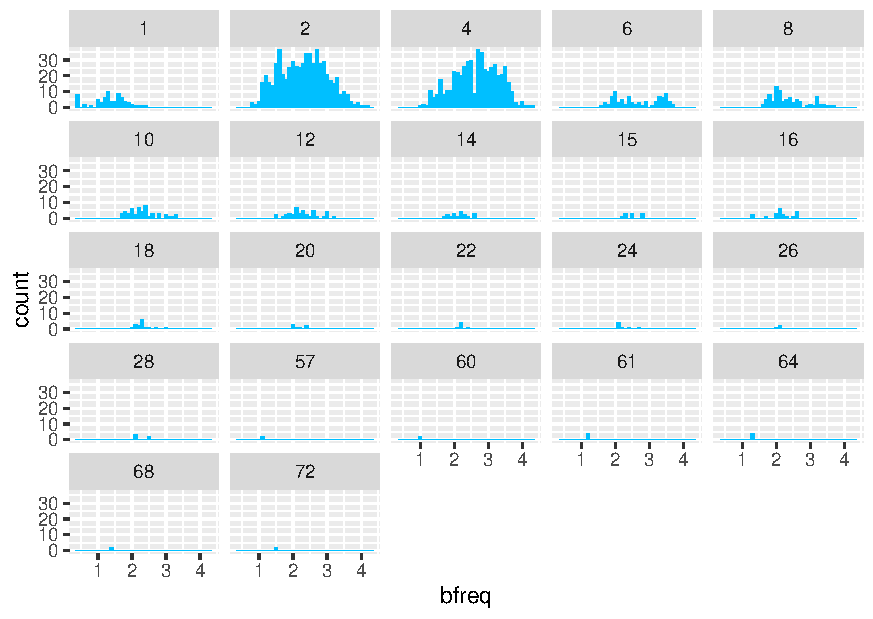
\includegraphics[width=0.5\textwidth]{./graphics/hist_bfreq_wrt_ncore.pdf}
    \caption{Base frequency distribution of each Group of core number}
    \label{fig:hist_bfreq_wrt_ncore}
\end{figure}

\textbf{NOTE: THERE IS A CODE REFERENCE HERE}

There are a wide range of core numbers in the industry provided by Intel. However, only 1, 2 and 4 cores are the most popular. Therefore, we keep 2 and 4 only,
while ignoring the rest. Note that the reason why we do not keep 1-core, 6-cores, 8-cores and 12-cores is that its frequencies are very small compared to 2 and 4.
One more reasonable motivation behind this decision is that some \textit{Lithography} may not exist in these category (multiple cores trend is only induced recently,
and lithography is heavily dependent on the era of which the CPU is launched), making it difficult to compare with other groups. Therefore, it is better to ignore it.

\textbf{NOTE: THERE IS A CODE REFERENCE HERE}

As a summary, we represent this boxplot between many variables, to have a broad view over what we have done so far:

\begin{figure}[H]
    \centering
    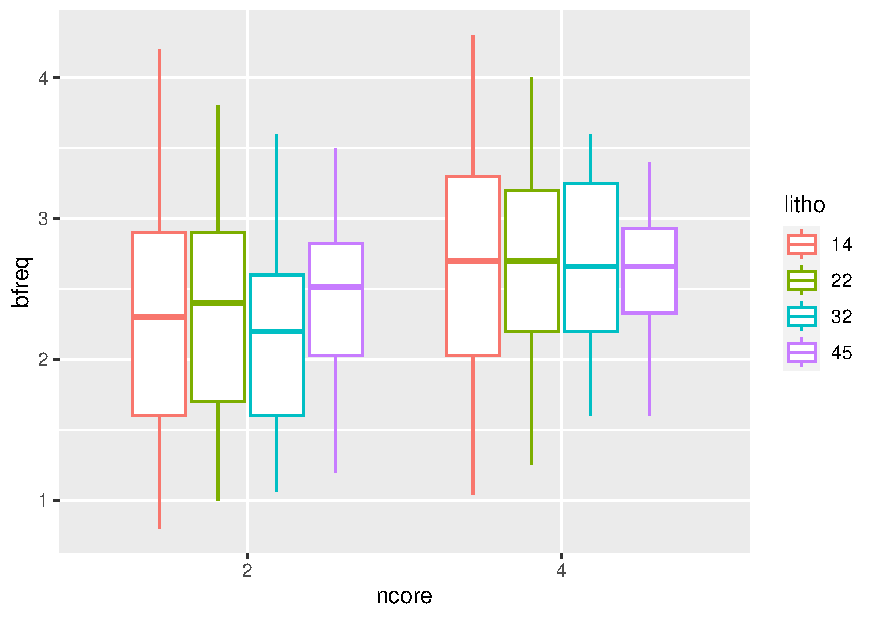
\includegraphics[width=0.5\textwidth]{./graphics/box_bfreq_wrt_ncore_litho.pdf}
    \caption{Box plot of Base frequency with respect to No. cores and Lithography}
    \label{fig:box_bfreq_wrt_ncore_litho}
\end{figure}

\textbf{NOTE: THERE IS A CODE REFERENCE HERE}




\subsubsection{Regression figures here, if any}